\documentclass{article}
\usepackage[OT1]{fontenc}
\usepackage{graphicx}
\usepackage{setspace}
\usepackage{anysize}
\usepackage{enumerate}
\usepackage{amssymb}
\usepackage{algorithm2e}
\usepackage{amsthm}
\usepackage{amsmath}
\usepackage{booktabs}
\usepackage{listings}
\usepackage{ulem}
\marginsize{3cm}{3cm}{0cm}{3cm}

\fontfamily{ptm}\fontsize{14}{14}\selectfont 
\singlespacing
\newcommand{\solution}[1]{~\\ $\blacksquare$ \sffamily\upshape\selectfont #1
\normalfont ~\\~ }
\newcommand\independent{\protect\mathpalette{\protect\independenT}{\perp}}
\def\independenT#1#2{\mathrel{\rlap{$#1#2$}\mkern2mu{#1#2}}} 
\setlength{\parindent}{0pt}
% \setlength{\textwidth}{1.5\textwidth}

\begin{document}
\begin{center}
\textbf{\large{
Introduction to Artifitial Intelligence \\
\small{Final Exam.}}} \\
\textsc{\Large{Shumin Guo}}
\end{center}

\textbf{Problem 1.}(10 points) Suppose Box 1 contains 10 apples and 5
oranges, and Box 2 contains 7 apples and 5 oranges. One of the boxes
is chosen at random (with equal probability) and an item is sellected
from the box and found to be an apple. Find the probability that the
apple came from Box 1.
\solution{
  Let's use A to denote apple, O to denote orange, B1 denotes from
  box1 and B2 denotes from box 2. 
  \begin{align*}
    P(B_1) & = P(B_2) = 0.5 \\ 
    P(A|B_1) & = \frac{10}{15} = \frac{2}{3} \\ 
    P(O|B_1) & = \frac{5}{15} = \frac{1}{3} \\ 
    P(A|B_2) & = \frac{7}{12} \\ 
    P(O|B_2) & = \frac{5}{12} \\
  \end{align*}
  The probability of from Box1 when get an apple is.
  \begin{align*}
    P(B_1|A) & = \frac{P(A|B_1)P(B_1)}{P(A)} \\
    & = \frac{P(A|B_1)P(B_1)}{P(A|B_1)P(B_1)+P(A|B_2)P(B_2)} \\
    & = \frac{\frac{2}{3}\times \frac{1}{2}}{\frac{2}{3}\times
      \frac{1}{2}+ \frac{7}{12}\times \frac{1}{2}} \\
    & = \frac{\frac{1}{3}}{\frac{1}{3}+\frac{7}{24}} \\ 
    & = \frac{8}{15} 
  \end{align*}
} 

\textbf{Problem 2.} (15 points) Consider a Bayesian network with the
following structure in Figure \ref{fig:final_2.1}.
\begin{figure}[ht]
  \centering
  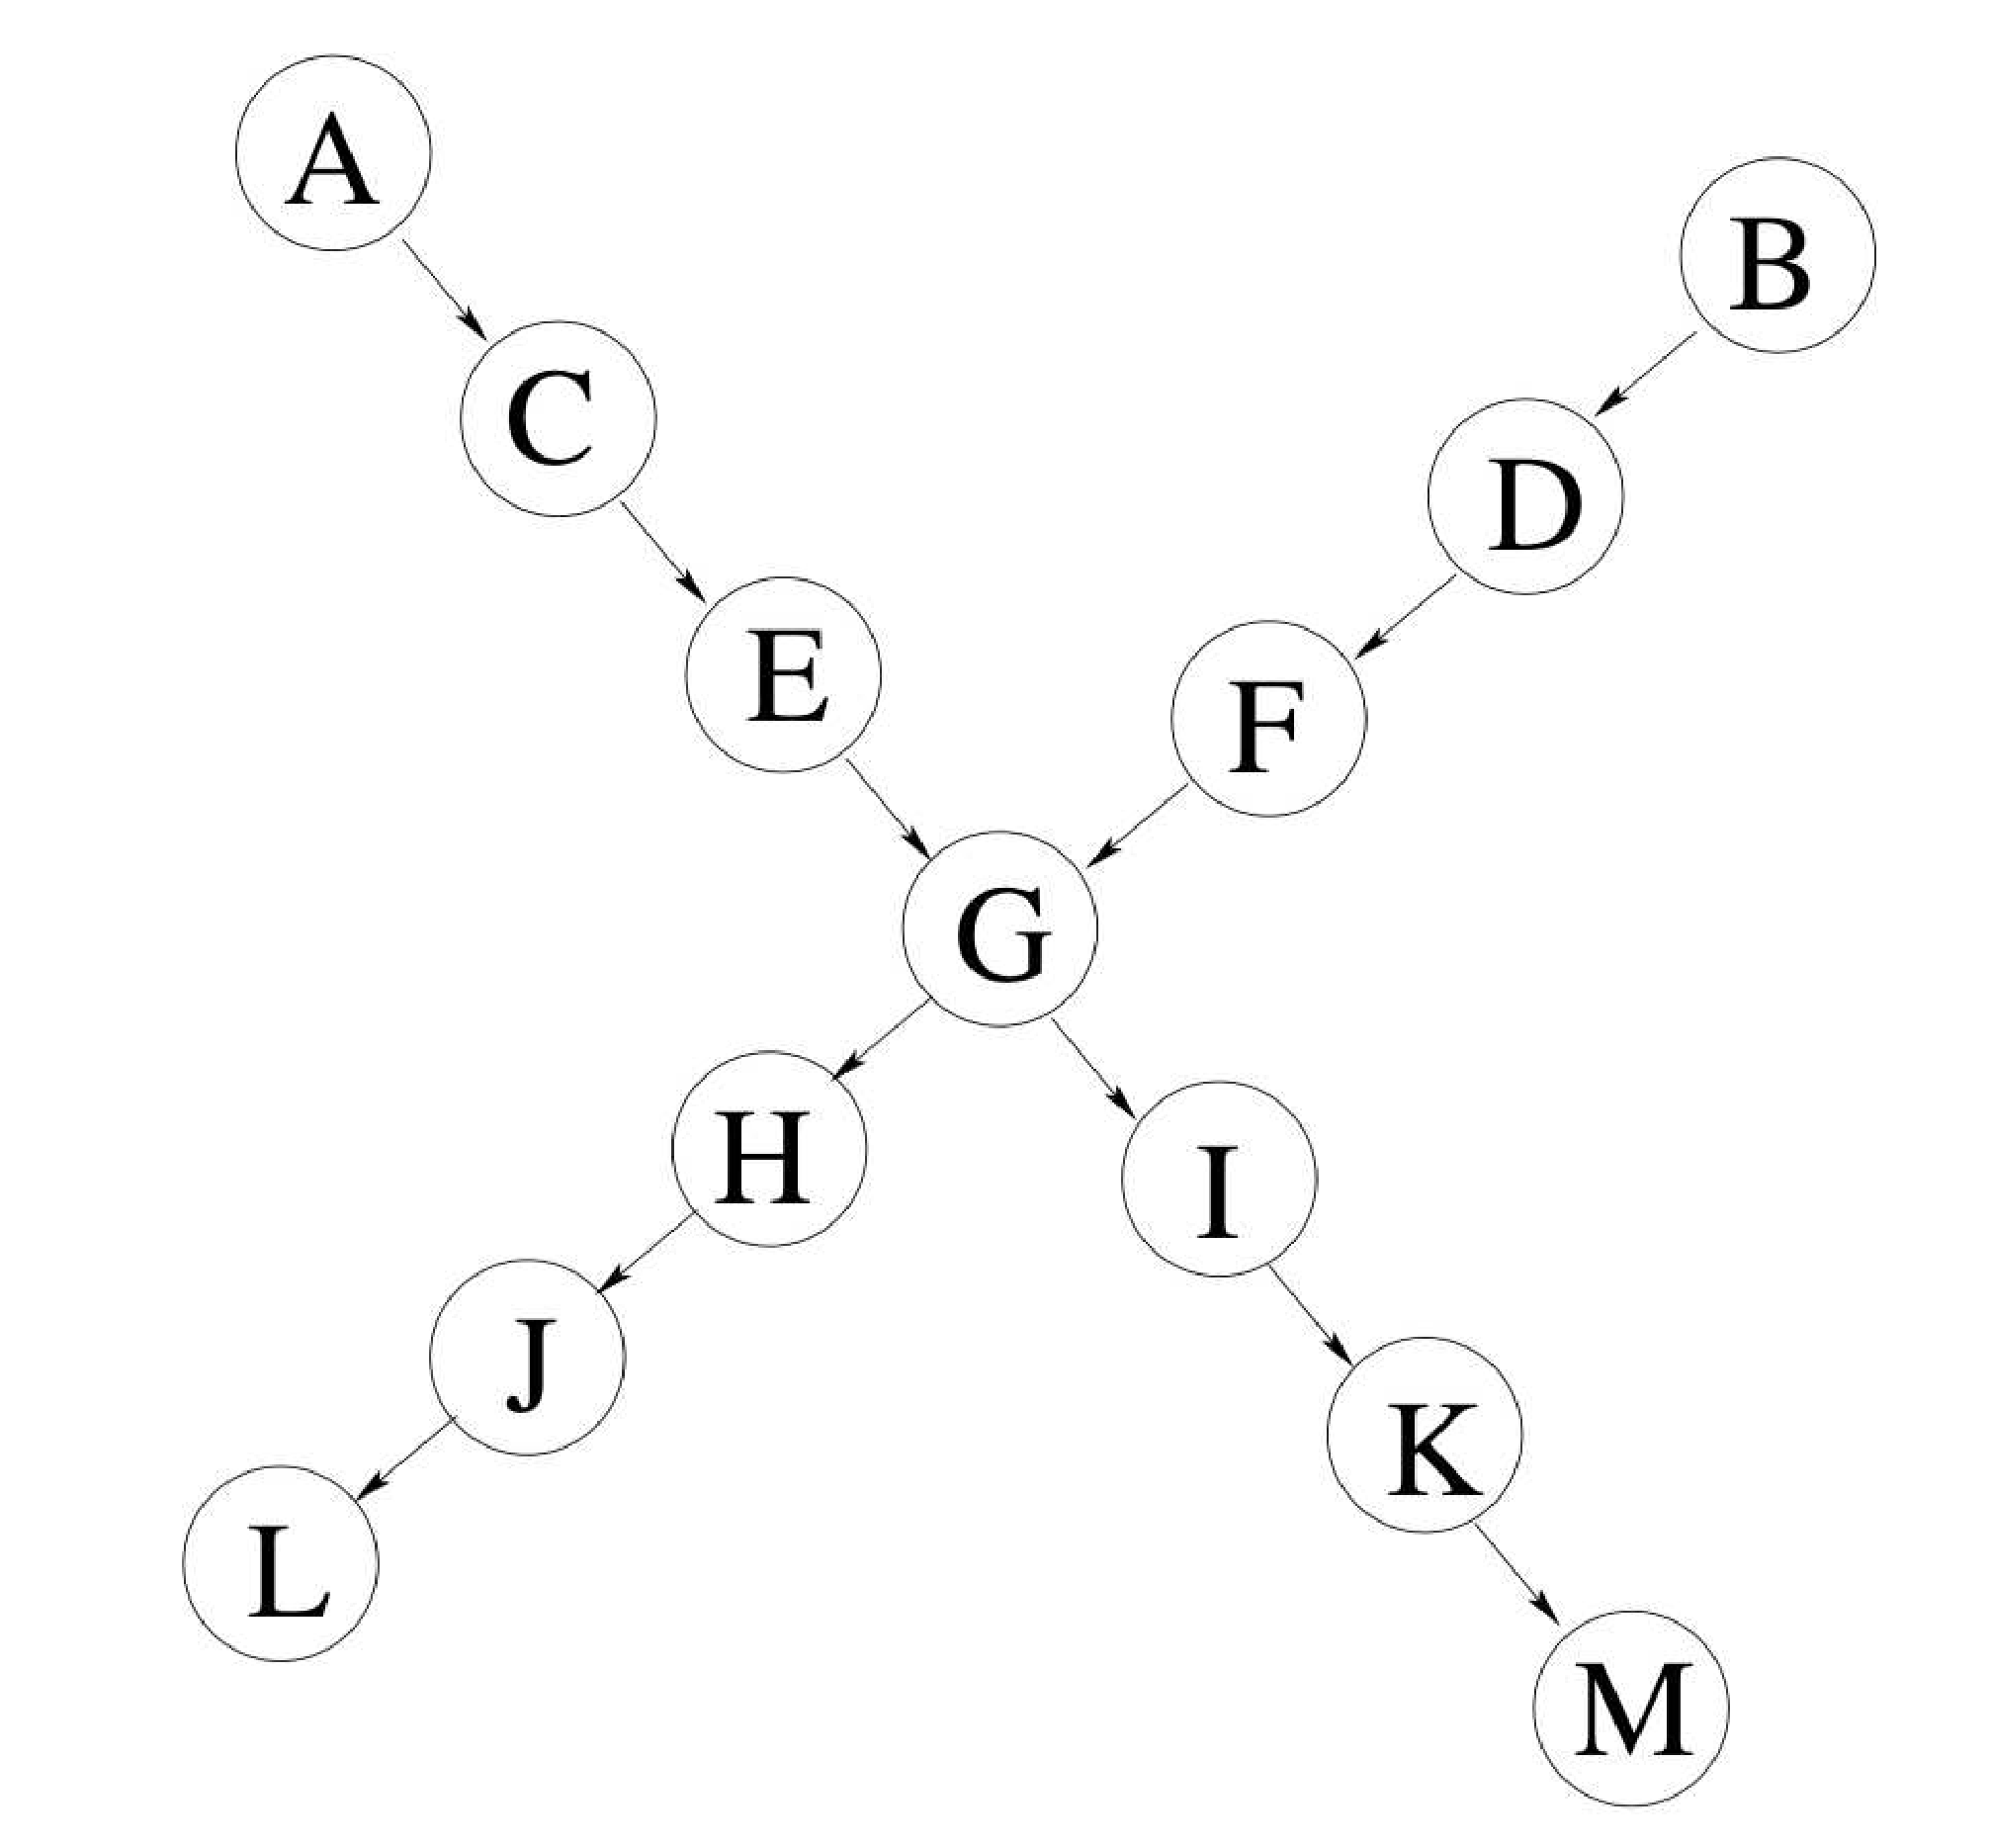
\includegraphics[width=.5\textwidth]{AI-FINAL-2_1.pdf}
  \caption{Bayesian Network for problem 2.}\label{fig:final_2.1}
\end{figure}
Does computing $p(M|A)$ depend on:
\begin{itemize}
  \item $p(L|J)?$
  \item $p(K|I)?$
  \item $p(D|B)?$
  \item $p(H|G)?$
\end{itemize}
In the network of Figure \ref{fig:final_2.1} if we decided not to
include G in our network, but still wanted to model the joint
distribution of all the other variables, what is the smallest network
structure we could use?
\solution{
  With the theory of d-seperation, any node on the path of $A\rightarrow M$
  will affact the computation of $p(M|A)$, so in the given choices,
  $p(K|I)$ has clearly sperate the path, which renders $p(M|A) =
  p(M)$, and for choice $p(H|G)$, the evidence of $G$ makes
  $A\independent H | G$ and $M\independent H | G$. And we have 
  $M\independent A | G$. 

  In the given Bayesian network, we have 
  \[ P(A,B,C...M) = P(A)P(B)P(C|A)P(D|B)P(E|C)P(F|D)
  P(G|EF)P(H|G)P(I|G)P(J|H)P(K|I)P(L|J)P(M|K) \]
  By removing node $G$, we can consider that $G$ becomes evident
  node. So, in this case, 
}

\textbf{Problem 3.} (25 points) Let $H_x$ be a random variable
denoting the handedness of an individual $x$, with possible values $l$
or $r$. A common hypothesis is that left- or right-handedness is
inherited by a simple mechanism; that is, perhaps there is a gene
$G_x$ , also with values $l$ or $r$, and perhaps actual handedness
turns out mostly the same with some probability $s = 0.95$ as the gene
an individual possesses. Furthermore, perhaps the gene itself is
equally likely to be inherited from either of an individual’s parents,
with a small probability $m = 0.05$ of a random mutation flipping the
handedness.
\begin{enumerate}[(a)]
\item Which of the three networks in Figure \ref{fig:final_3.1} claim
  the following?
  \begin{figure}[ht]
    \centering
    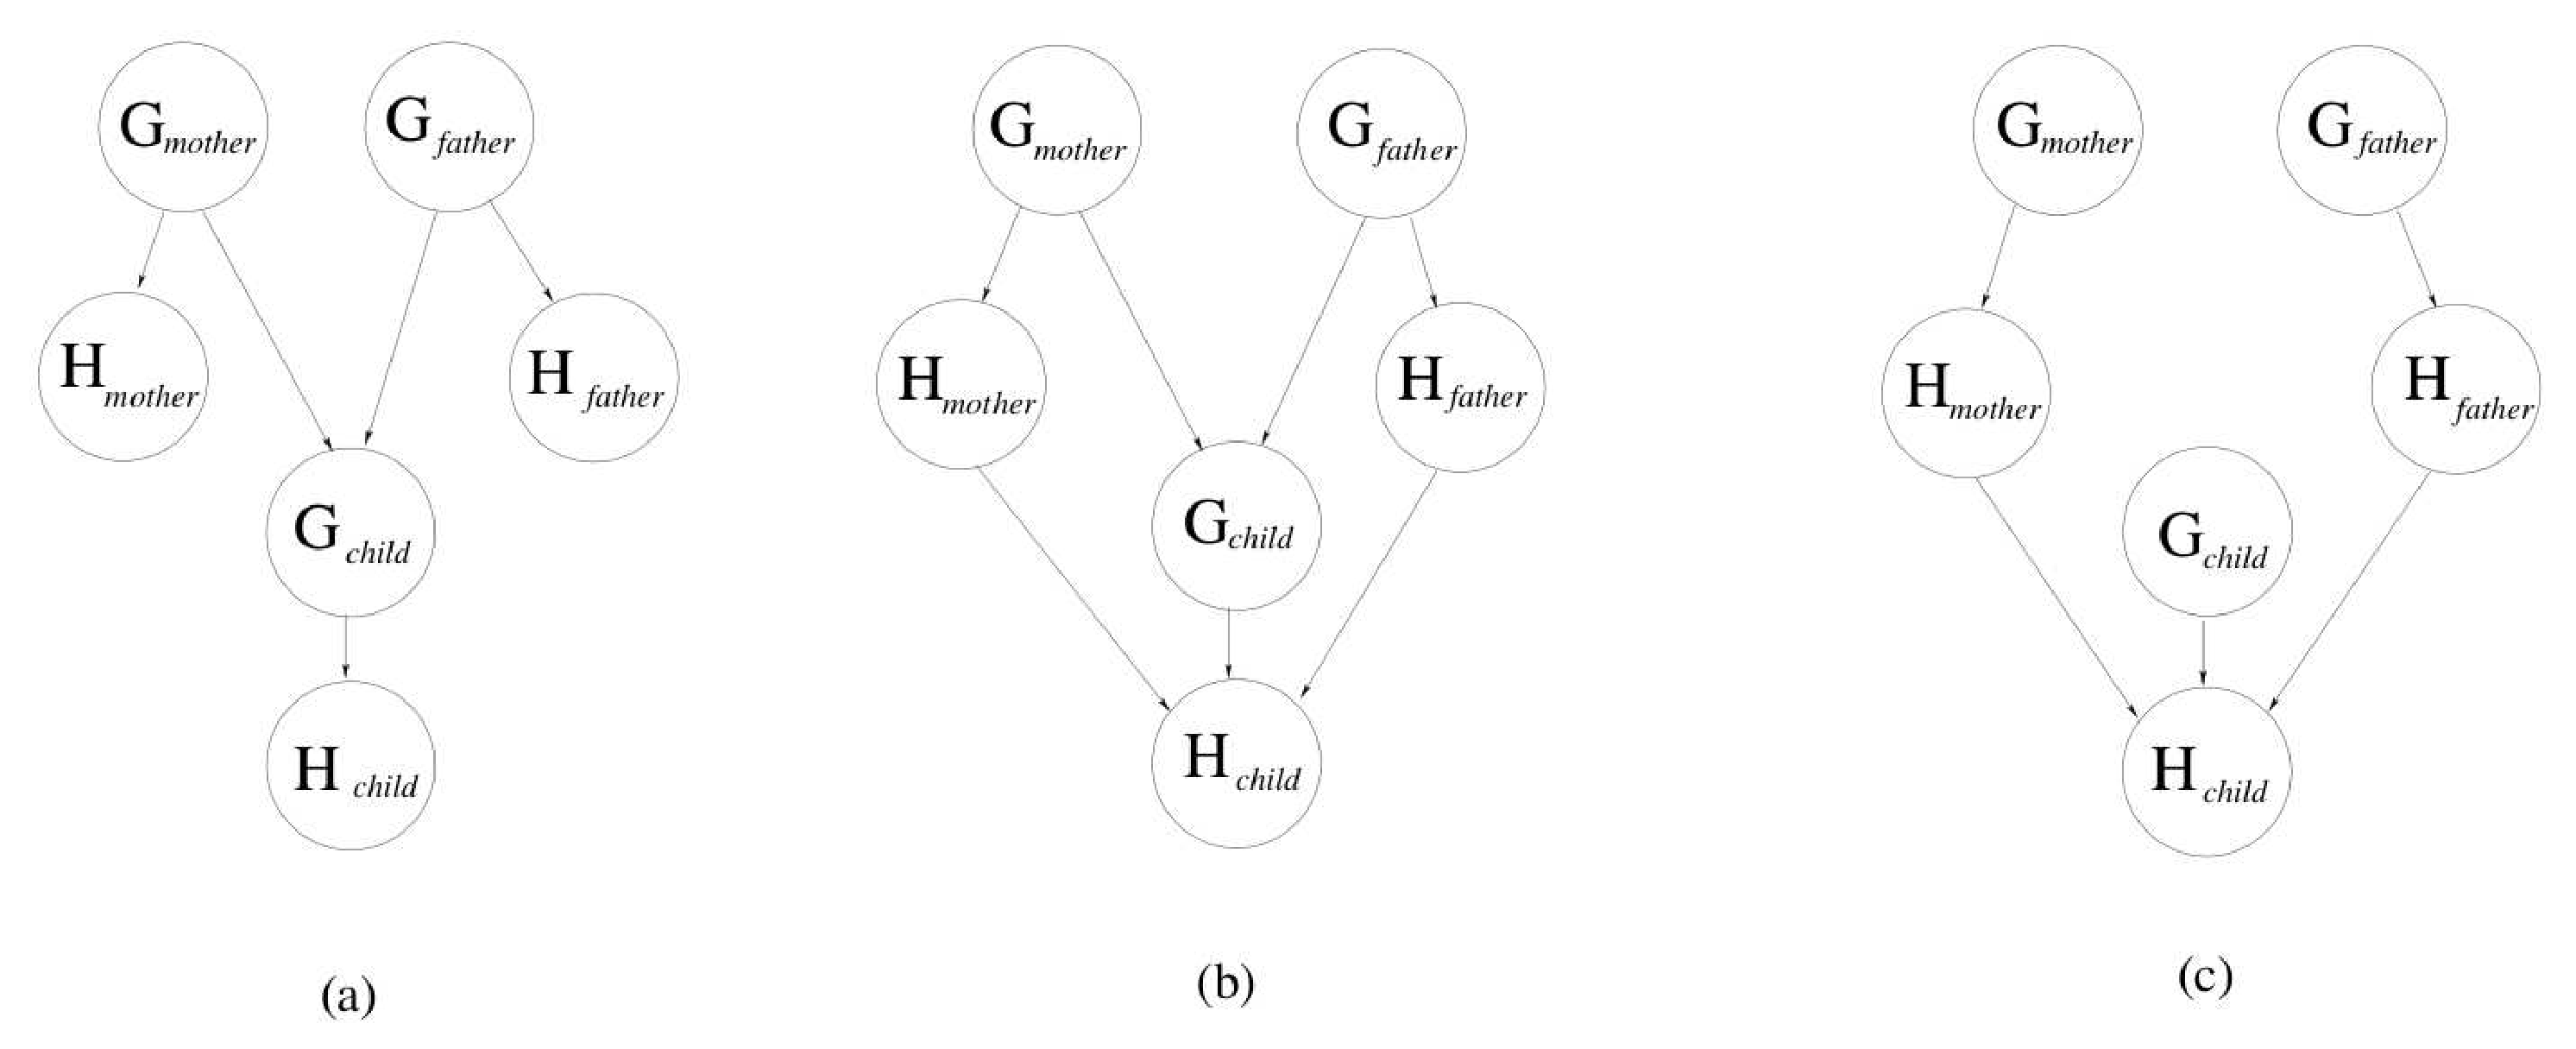
\includegraphics[width=.8\textwidth]{AI-FINAL-3_1.pdf}
    \caption{Bayesian Network for problem 3.}\label{fig:final_3.1}
  \end{figure}
  \[ P(G_{father}, G_{mother}, G_{child}) =
  P(G_{father})P(G_{mother})P(G_{child}) \]
  Please explain.
\solution{
  c. Because only figure (c) claims that $G_{father}, G_{mother},
  G_{child}$ are independent without any given information. And for
  (a) and (b) $G_{child}$ is dependent on $G_{father}, G_{mother}$. 
}
\item Which of the three networks make independence claims that are
  consistent with the hypothesis about the inheritance of handedness?
  Please explain.
\solution{
  a. According to the problem hypothesis, handness of fathers and
  mothers can not directly influence that of the child, so only (a)
  can claim this hypothesis. 
}
\item Which of the three networks is the best description of the
  hypothesis? Please explain.
\solution{
  a. Similar the the above question. Handness of fathers and
  mothers can not directly influence that of the child, only handness
  gene has direct influence on the handness of child.
}
\item Write down the $CPT$s for the $G_{child}$ node and $H_{child}$ node in
  network (a), in terms of $s$ and $m$.
  \solution{}
    CPT for $G_{child}$, $G_{cl}$ means child has left hand side
    gene. Other notations are similar. 
    \begin{align*}
      P(G_{cl}|G_{fl},G_{ml}) & = 1-m = 0.95\\
      P(G_{cl}|G_{fl},G_{mr}) & = 0.5\times (1-m) + 0.5\times m = 0.5 \\ 
      P(G_{cl}|G_{fr},G_{ml}) & = 0.5\times m + 0.5\times (1-m) = 0.5 \\ 
      P(G_{cl}|G_{fr},G_{mr}) & = 0.5\times m + 0.5\times m = m = 0.05 
    \end{align*}

    CPT for $H_{child}$. 
    \begin{align*}
      P(H_l|G_l) & = P(H_r|G_r) = s = 0.95 \\ 
      P(H_l|G_r) & = P(H_r|G_l) = 1-s = 0.05 \\ 
    \end{align*}

\item Suppose that $p(G_{mother} = l) = p(G_{father} = l) = 0.5$. In
  network (a), what is the value of $p(G_{child} = l)$? What is the
  value of $p(H_{child} = l)$? 
\solution{
  \begin{align*}
    p(G_{cl}) & = \sum_{x\in \{l,r\}}\sum_{y\in \{l,r\}}p(G_{cl}G_{fx}G_{my})\\ 
    & = P(G_{cl}|G_{fl},G_{ml})P(G_{fl})P(G_{ml}) + 
    P(G_{cl}|G_{fl},G_{mr}) P(G_{fl})P(G_{mr}) \\
    & + P(G_{cl}|G_{fr},G_{ml})P(G_{fr})P(G_{ml}) + 
    P(G_{cl}|G_{fr},G_{mr})P(G_{fr})P(G_{mr}) \\ 
    & = 0.95\times 0.5\times 0.5 + 0.5\times 0.5\times 0.5 + 
    0.5\times 0.5\times 0.5 + 0.05\times 0.5\times 0.5\\ 
    & = 0.25\times 2 \\ 
    & = 0.5 \\ 
    & \\
    P(H_{cl}) & = \sum_{x\in\{l,r\}}P(H_{cl}G_{cx}) \\ 
    & = P(H_{cl}|G_{cl})P(G_{cl}) + P(H_{cl}|G_{cr})P(G_{cr}) \\ 
    & = 0.95\times 0.5 + 0.05\times 0.5 \\ 
    & = 0.5
  \end{align*}
}
\item Again suppose that $p(G_{mother} = l) = p(G_{father} = l) =
0.5$. In network (a), suppose we observe the value of $H_{child}$ is r,
what is the most likely value of $G_{mother}$ you can infer from this
observation?
\solution{
  I will compute the most likelihood value of $P(G_{mr}|H_{cr})$ which is the
  probability that mother has right hand gene.
    \[ P(G_{mr}|H_{cr}) =
    \sum_{x,y,z\in\{l,r\}}P(G_{mr},G_{fx},H_{my},H_{fz},G_{cw}|H_{cr})
    \]
}
\end{enumerate}

\textbf{Problem 4}. (25 points) Let $P(A) = \phi, P (B) = \mu, P (C) =
2\mu, P (D) = 1 - \phi - 3\mu$ denotes the probability of getting A,
B, C and D grade in a class respectively. We want to estimate $\phi$ and $\mu$
from data. 
\begin{enumerate}
\item Assume in a given class, there were $a = 14$ students getting
  As, $b = 6$ students getting Bs, $c = 9$ students getting Cs, and $d
  = 10$ students getting Ds. What is the maximum likelihood estimate of
  $\phi$ and $\mu$?
\solution{
  The likelihood function can be represented as follows: 
  \begin{align*}
    P(A,B,C,D|\mu, \phi) & = \phi^a\mu^b(2\mu)^c(1-\phi-3\mu)^d \\
    LL & = alog\phi + blog\mu + c\log2\mu + dlog(1-\phi-3\mu) \\
    \frac{\partial LL}{\partial \mu} &= \frac{b}{\mu} + \frac{c}{\mu}
    - \frac{3d}{1-\phi-3\mu} = 0 \\
    &\Rightarrow \frac{b+c}{\mu} - \frac{3d}{1-\phi-3\mu} = 0 \\ 
    \frac{\partial LL}{\partial \phi} &= \frac{a}{\phi} -
    \frac{d}{1-\phi-3\mu} = 0 \\ 
    &\Rightarrow \mu = \frac{b+c}{3(a+b+c-d)},~\phi = 
    \frac{a(a-d)}{(a+d)(a+b+c-d)} \\ 
    &\Rightarrow \mu = \frac{5}{19}\approx 0.263157895, ~ \phi =
    \frac{7}{57} \approx 0.122807018 \\
  \end{align*}
}
\item Someone tells you that the number of high grades (As + Bs) is $h
= 20$, and the number of low grades (Cs + Ds) is $g = 19$. What is the
maximum likelihood estimate of $\phi$ and $\mu$ now? Please use EM
algorithm to obtain the answer. Is your result a global maximum or
local maximum? Please justify and explain why.
\solution{
  In the E-step, by using the prior probabilities of $a, b, c, d$ we
  have: 
  \begin{align*}
    a & = \frac{\frac{\phi}{\mu}}{1+\frac{\phi}{\mu}}h \\ 
    b & = \frac{h}{1+\frac{\phi}{\mu}} \\ 
    c & = \frac{2\mu}{1-\phi-\mu}g \\ 
    d & = \frac{1-\phi-3\mu}{1-\phi-\mu} g
  \end{align*}
  M-step: \\
  By combining the expected value of $\mu$ and $\phi$ from the
  previous questions and the expected values of $a,b,c,d$, we can get
  the maximum likelihood value of $\mu$ and $\phi$ as follows: 
  \begin{align*}
    \mu & = \frac{b+c}{3(a+b+c-d)} \\
    %  =\frac{\frac{h}{1+\frac{\phi}{\mu}}+\frac{2\mu g}{1-\phi-\mu}} 
    % {3(h+\frac{2\mu g}{1-\phi-\mu}-\frac{(1-\phi-3\mu)g}{1-\phi-\mu})} \\ 
    % & = \frac{\frac{20}{1+\frac{\phi}{\mu}}+\frac{38\mu}{1-\phi-\mu}} 
    % {3(20+\frac{19(5\mu+\phi-1)}{1-\phi-\mu})} \\
    \phi & = \frac{a(a-d)}{(a+d)(a+b+c-d)}
  \end{align*}
  And by iteratively applying the E-step and M-step, after iterating for 20
  rounds, the value converges to: 
  \ttfamily\selectfont{
    h = 20; \\ 
    g = 19; \\
    u = 10; \\
    p = 10; \\
    i = 1:50; \\
    for x = i,\\
    a = (p * h / u ) / (1 + p / u); \\
    b = h / (1 + p / u);\\
    c = 2 * u * g / (1 - p - u); \\
    d = (1 - p - 3 * u); \\
    
    u = (b + c) / (3 * (a + b + c -d));\\
    p = a * (a - d) / ((a + d) * (a + b + c - d));\\
    
    u, p\\
    endfor;}\normalfont

  \begin{align*}
    \mu & = 0.24349 \\
    \phi & = 0.26952
  \end{align*}
  This is global maximum, changing the initial values does not affect the
  result. 
}
\end{enumerate}

\textbf{Problem 5}. (25 points) Consider an HMM of a coin-tossing
experiment, assume a three-state model (corresponding to three
different coins) with probabilities and with all state-transition
probabilities 
\begin{table}[h]
  \centering
  \begin{tabular}{cccc}
    \toprule
    & \textbf{State 1} & \textbf{State 2} & \textbf{State 3} \\ \toprule
    $p(H)$ & $0.5$ & $0.75$ & $0.25$ \\ \midrule
    $p(T)$ & $0.5$ & $0.25$ & $0.75$ \\ \bottomrule
  \end{tabular}
  \caption{Sample data using XOR function.}
  \label{tbl:1-f}
\end{table}

equal to $\frac{1}{3}$. (Assume initial state probabilities of $\frac{1}{3}$).
\begin{enumerate}[a.]
\item You observe the sequence $O = (HHHHTHTTTT)$, what state sequence
  is most likely? What is the probability of the observation sequence
  and this most likely state sequence?
\solution{
  We need to calculate the forward message: 
  \begin{align*}
    \alpha_t(i) & = P(O_1,O_2,\ldots,O_t \wedge q_t) = S_i|\lambda, 
    1\leq t \leq T. \\ 
    & = \sum_iP(q_{t+1}=S_j|q_t=S_i)P(O_{t+1}|q_{t+1}=S_j)\alpha_t(i) \\ 
    & = \sum_i\alpha_{ij}b_j(O_{t+1})\alpha_t(i) \\
    & = 0.00010.
  \end{align*}
  The most likely state sequence is $2,2,2,2,3,2,3,3,3,3$. 
}
\item What is the probability that the observation sequence came
  entirely from state 1? 
\solution{
  \begin{align*}
    P(HHHHTHTTTT|1111111111) & = P(S_1)\prod_{i=1}^{10}P(O_i|S_i)P(S_i|S_{i-1}) \\
    & = 0.0000000017. 
  \end{align*}
}
\item Consider the observation $O = (HTTHTHHTTH)$, how would your answer to parts a and b
change? 
\solution{
  Similar to question 5.(a), and by calculation the forward information, we can get the
  most likely state sequence as $2,3,3,2,3,2,2,3,3,2$.
  And similar to question 5.(b), $P(HHHHTHTTTT|S) = 0.0000000026$.
}
\item If the state-transition probabilities were: $a_{11} = 0.9, a_{12} =
  0.05, a_{13} = 0.05, a_{21} = 0.45, a_{22} = 0.1, a_{23} = 0.45,
  a_{31} = 0.45, a_{32} = 0.45, a_{33} = 0.1$, how would your answers
  to parts a-c change? What does this suggest about the type of
  sequence generated by the models? 
\solution{
  For (a), the observation sequence is $HHHHTHTTTT$, $P(HHHHTHTTTT) = 0.00009.$
  The most likely sequence is $2,1,1,1,1,1,1,1,1,1$. \\
  For (b), the forward information sequence is $0.000013$. \\ 
  
  For observation $O=(HTTHTHHTTH)$, by using the similar method, we get the most likely
  sequence as $2,3,1,1,1,1,1,1,1,1$.
}
\end{enumerate}
\end{document}